\section{Jets: Quarks and Gluons}
Collisions of high energy particles with hadrons, produce jets of new hadrons or other particles. 

\subsection{Evidence for 3 Quark Colors}
\begin{itemize}
    \item The ratio $R$ between the cross-sections of producing hadrons in $e^+e^-$ collisions, compared to the cross-section of producing muons, show how many quark colors are possible. 
    \begin{equation}
      R ≡ \frac{σ(e^+e^- → \text{hadrons})}{σ(e^+e^- → μ^+μ^-)}
    \end{equation}
    The cross-section for producing hadrons is the sum of the cross-sections for producing quark-antiquark pairs with an center-mass energy too high to be produced. We must also take into account the number of colors $N_c$. 
    \begin{equation}
      σ(e^+e^- → \text{hadrons}) = ∑_{f}^{} σ(q_f \bar{q}_f) = ∑_{f}^{} N_c e^2_{f} σ(e^+e^- → μ^+μ^-)
    \end{equation}
    \begin{equation}
      R_0 ≡ N_c (e^2_{u} + e^2_{d} + e^2_{s} + e^2_{c} + e^2_{b} + e^2_{t}) = \frac{11}{9}N_c 
    \end{equation}
    Adding the gluon radiation we make a small correction. 
    \begin{equation}
      R_{\text{theory}} = R_0 \left(1 + \frac{α_s}{π}\right)
    \end{equation}
    \item The experimental values show that $N_c$ must be 3.
\end{itemize}


\subsection{Di-jet Production at $p p$ (\cref{fig: di-jet_production})}
\begin{figure}[h!]
\centering
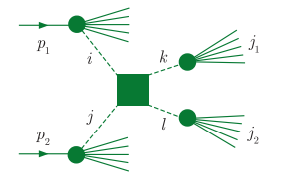
\includegraphics[width = .45\textwidth]{di-jet_production.png}
\caption{Dominant mechanism for di-jet production in $pp$ collisions.}
\label{fig: di-jet_production}
\end{figure}


\subsubsection{Rapidity}
Useful as $y_1 - y_2$ is lorentz invariant. 
\begin{equation}
  y = \frac{1}{2} \ln \left(\frac{E + p_z}{E - p_z}\right)
\end{equation}
\subsubsection{Pseudorapidity}
Practical high-energy approximation when you do not know everything about all particles. 
\begin{equation}
  η = -\ln \left(\tan \left(\frac{θ}{2}\right)\right)
\end{equation}

\subsubsection{Transverse Momentum}
When looking at collisions, we expect the transverse momentum to be zero. If this is not the case, it means some particle we did not detect, has taken some of the momentum.

\subsection{Current and Constituent Quarks}
\begin{itemize}
  \item The static quark model of hadrons consider them just staying still. 
  \item QCD is a dynamic theory, where quarks move at relativistic speeds, which affects their interactions with the gluons. 
  \item The masses of the quarks depends on their environment and what model is being used. Just as the coupling constants, they too run. 
  \item The mass of the proton comes from the interactions between the quarks through the strong force. The Higgs interataction contributes far less. 
\end{itemize}


\section{Weak Interactions and Electroweak Unification}
\begin{itemize}
  \item Untill 1973, we had only observed charged weak interactions, through the $W^{\pm}$-boson. We had already unified the electromagnetic and weak interactions (electroweak interactions) since the 1960s.
  \item It was nearly impossible to create a model with only the $W^{\pm}$-boson and the photon.
  \item The Brout-Englert-Higgs (BEH) predicted a neutral, heavy boson, the $Z^0$-boson.
  \item The neutral interactions were predicted to be found 1/3 as often as the charged interactions, which was later observed. 
\end{itemize}

\subsection{Low and High Energy Weak Interactions}
\begin{itemize}
  \item The invariant amplitude for Yukawa potential:
  \begin{equation}
    \mathcal{M} = \frac{g^2ℏ^2}{Q^2 - M^2c^2}
  \end{equation}
  shows that when momentum transfer $Q^2$ goes to zero, the great mass of the weak bosons makes the amplitude small. 
  \item This is the reason why the weak force is short-ranged.
  \item At low energies, the electromagnetic and weak forces can be seen as separate. 
  \item At high energies, the contribution to the Yukawa potential is about the same, and the forces can be seen as one.
\end{itemize}

\subsection{Charged Weak Interactions}
\subsubsection{Basic Principles}
\begin{itemize}
  \item \textbf{Lepton Universality}: The weak interactions are the same for all flavours.
  \item \textbf{Lepton-Quark Symmetry}: The coupling of the $W^{\pm}$ to leptons and all quarks are the same.
  \item \textbf{Quark Mixing}: The quark eigenstates (') are linear combinations of mass/strong-force eigenstates. 
  \begin{equation}\label{eq: quark_mixing}
    \begin{pmatrix}
      d' \\ s' \\ b'
    \end{pmatrix}
    = 
    \begin{pmatrix}
      V_{ud} & V_{us} & V_{ub} \\
      V_{cd} & V_{cs} & V_{cb} \\
      V_{td} & V_{ts} & V_{tb}
    \end{pmatrix}
    \begin{pmatrix}
      d \\ s \\ b
    \end{pmatrix}
  \end{equation}
\end{itemize}

\subsection{Quark Mixing}
\begin{itemize}
  \item Pions decay relatively slow via $π^{+} → μ^{+} ν_{μ}$
  \item This is the same as $u \bar{d} → μ^{+} ν_{μ}$ or $u \bar{d} → W^{+} → μ^{+} ν_{μ}$. 
  \item Kaons decay, with a long lifetime as well via $K^{+} →  μ^{+} ν_{μ}$. As a kaon is $u \bar{s}$ which is neither $u \bar{d}$ nor $c\bar{s}$, this means there must be some mixing. We can hypothesize that the weak and strong eigenstates of the quarks are not necessarily the same. 
  \item Using the same mixing hypothesis as for neutrino mixing, we believe mass eigenstates are mixtures of flavour eigenstates. 
  \begin{equation}
    \begin{pmatrix*}[r]
     d' \\
     s' \\
    \end{pmatrix*}  = 
    \begin{pmatrix*}[r]
      \cos θ_c & \sin θ_c \\
      -\sin θ_c & \cos θ_c \\
    \end{pmatrix*}
    \begin{pmatrix*}[r]
      d \\
      s \\
    \end{pmatrix*} = 
    \begin{pmatrix*}[r]
     V_{ud} & V_{us} \\
     V_{cd} & V_{cs} \\
    \end{pmatrix*} 
    \begin{pmatrix*}[r]
      d \\
      s \\  
    \end{pmatrix*}
  \end{equation}
\end{itemize}
\subsubsection{Examples}
$θ_{c}$ is the Cabibbo angle.
\paragraph{Pion}
\begin{equation}
u \bar{d}' = W^{+} → μ^{+} ν_{μ}
\end{equation}
\begin{equation}
  d' = d \cos θ_c + s \sin θ_c
\end{equation}
\begin{equation}
  u \bar{d} = W^{+} → μ^{+} ν_{μ}
\end{equation}
\paragraph{Kaon}
\begin{equation}
  u \bar{s}' → W^{+} → μ^{+} ν_{μ}
\end{equation}
\begin{equation}
  s' = -d \sin θ_c + s \cos θ_c
\end{equation}